%author: Pedro Pinto; v2.1; November 2019
\documentclass[a4paper]{report}
\usepackage[utf8]{inputenc}
\usepackage{amsmath}
\usepackage{graphicx}
\usepackage{tabularx}
\usepackage{adjustbox}
%\usepackage[colorinlistoftodos]{todonotes}
\usepackage{csquotes}
\usepackage{comment}
\usepackage{imakeidx}
%tabela
\usepackage{multirow}
\usepackage{xcolor}
\usepackage[margin=3cm]{geometry}
\usepackage[hidelinks]{hyperref} %to show links
\usepackage[toc,acronym,nopostdot,nonumberlist]{glossaries}
\usepackage{titling}
\usepackage{tikzpagenodes}
\usepackage[ddmmyyyy]{datetime}
\usepackage{setspace}
\usepackage{indentfirst}
\usepackage{rotating}

%para definir a localização das tabelas e imagens em modo strict
%\usepackage{placeins}

\usepackage[backend=bibtex]{biblatex}
\addbibresource{ref.bib}
\makeglossaries
\doublespacing

\begin{document}
	
	\begin{titlepage}
		\begin{center}
			\textsc{ \LARGE{Università della Svizzera Italiana \\}}
			\textsc{ \LARGE{Master of Science in Informatics\\ }}
			\vspace{30mm}
			\fontsize{10mm}{7mm}\selectfont 
			\textup{Software Engineering\\Assignment 8}\\
			\vspace{70mm}
		\end{center}
		
		\vspace{25mm}
		
		\begin{minipage}[t]{0.47\textwidth}
		\end{minipage}\hfill\begin{minipage}[t]{0.47\textwidth}\raggedleft
			\textnormal{\large{\bf Student:\\}}
			{\large Matteo Basso\\matteo.basso@usi.ch}
		\end{minipage}
		
		\vspace{20mm}
		
		\centering{\large{Academic year 2019/2020 \\ Lugano - \today }}
		
	\end{titlepage}
	
	%insert index
	\tableofcontents
	\glsaddall
	\printglossary[type=\acronymtype]
	\printglossary[type=main,title={Glossary},toctitle={Glossary}]
	%%%%%%%%%%%%%%%%%%%%%%%%%%%%%%%%%%%%%%%%%%%%%%%%%%%%%  
	
	\chapter{Introduction}
	\label{chap:introduction}
	
	This report summarizes the functionalities, choices, architecture and patterns that characterize the project. In this chapter general but fundamental information is provided, like the choice of the ORM library and the links to resources.
	
	\section{Context}
	\label{sec:context}
	
	The provided application implements the requirements specified by the text of the assignment, summarized here:
	
	\begin{itemize}
		\item Users can and must login in order to use the application.
		\item At least the first user must use the registration page before logging in.
		\item After the authentication it is possibile to perform CRUD (create, read, update, delete) operations for the entity that represents the user.
		\item Users can also be searched by:
			\begin{itemize}
				\item Username
				\item Name
				\item Best friend
				\item Country
				\item City
				\item Street
		\end{itemize}
	\end{itemize}

	\section{Hibernate}
	\label{sec:hibernate}
	
	In order to develop the application it has been decided to import Hibernate \cite{site:hibernate}, a popular ORM framework for Java. Using a library like this has multiple benefits in a real project, here are some of them:
	
	\begin{itemize}
		\item The sophisticated design of the data mapping layer is alleviated.
		\item It allows the usage of design patterns without implementing them from scratch. For example, Lazy loading or transactions can be used in a very simple and intuitive way.
		\item It handles edge cases in a better and tested way.
		\item Developers can think about the architecture of the system without worrying about these implementations.
		\item It assures the security of the system by default (for example, protecting from SQL Injection).
	\end{itemize}
	
	\section{Resources}
	\label{sec:resources}
	
	Code, report, diagrams and images are available in the GitHub Repository \cite{site:githubrepository} of the assignment:
	
	\begin{itemize}
		\item Servers and implementation are available in the \texttt{/code} folder.
		\item Diagram sources can be found in \texttt{/code/assignment8/diagrams} and can be opened using a working installation of IntelliJ IDEA Ultimate version.
		\item This document is available at \texttt{/report}.
		\item Diagrams and screenshots are located in \texttt{/report/images}.
	\end{itemize}

	\chapter{Application}
	\label{chap:application}
	
	In the following chapter, a brief explanation of the different pages is provided.
	
	\section{Login}
	\label{sec:login}
	
	A login is needed in order to use the application and access its functionalities. For this reason, every user must authenticate himself as a first step. This page is shown in figure \ref{fig:login}.
	
	\section{Registration}
	\label{sec:registration}
	
	Users can login into the system after submitting a registration. The following page, provide a way to do so, inserting some general information. This page is shown in figure \ref{fig:registration}.
	
	\section{User list}
	\label{sec:user_list}

	The first page of the application shows the list of registered users. It is possible to edit and delete each of them, except the one that is logged in. It is also possible to navigate to other pages and eventually logout. This page is shown in figure \ref{fig:user_list}.
	
	\section{User creation}
	\label{sec:user_creation}
	
	Users can be created also by another user without using the registration page. The form is the same. This page is shown in figure \ref{fig:new_user}.
	
	\section{User update}
	\label{sec:user_update}
	
	A user can also update every other using the same (precompiled) form showed before. This page is shown in figure \ref{fig:update_user}.
	
	\section{User search}
	\label{sec:user_search}
	
	Through a simple view, it is possible to search users. Filters are combined only if not empty. This page is shown in figure \ref{fig:search_user}.
	
	\begin{figure}[ht]
		\centering
		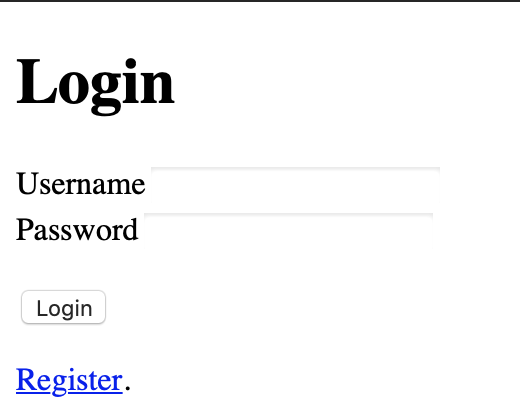
\includegraphics[scale=0.7]{images/login.png}
		\caption{Login page}
		\label{fig:login}
	\end{figure} 
	
	\begin{figure}[ht]
		\centering
		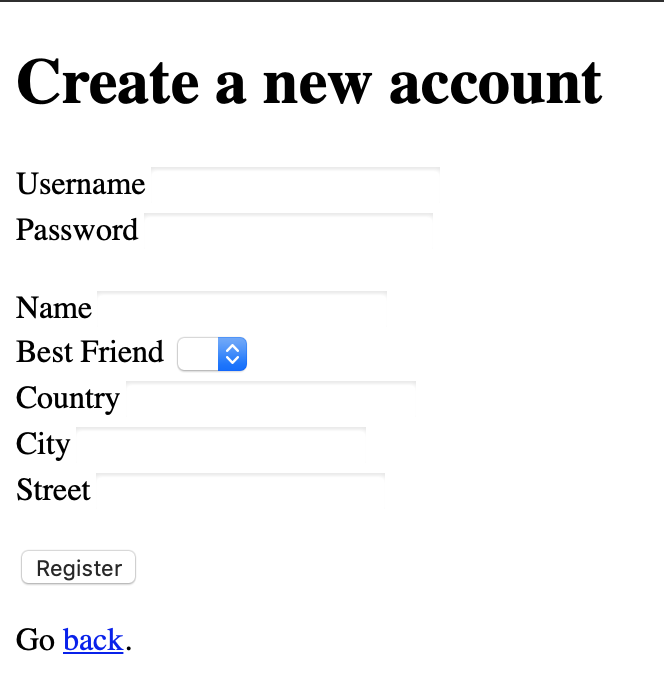
\includegraphics[scale=0.7]{images/registration.png}
		\caption{Registration page}
		\label{fig:registration}
	\end{figure}
	
	\begin{figure}[ht]
		\centering
		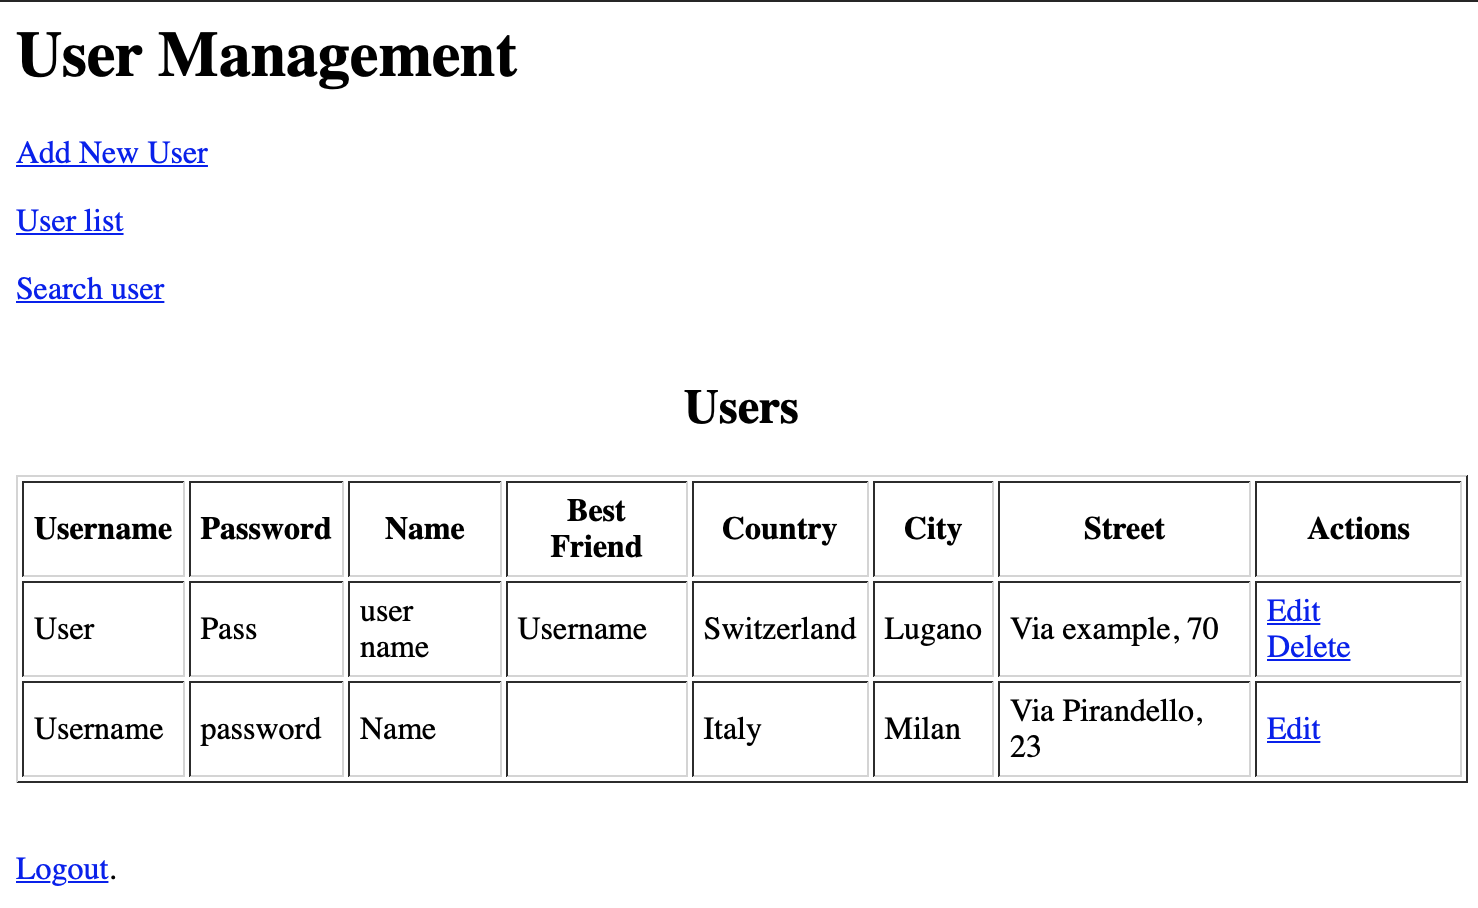
\includegraphics[scale=0.6]{images/userlist.png}
		\caption{User list page}
		\label{fig:user_list}
	\end{figure} 
	
	\begin{figure}[ht]
		\centering
		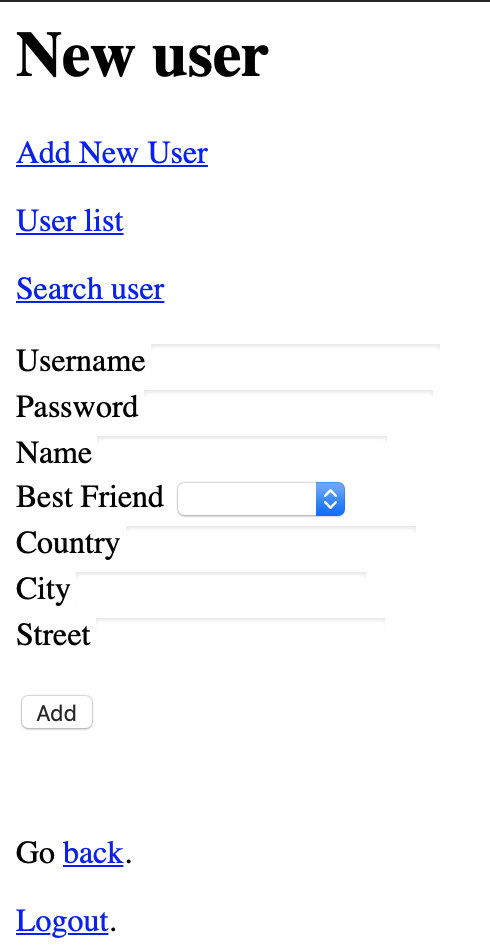
\includegraphics[scale=0.7]{images/newuser.png}
		\caption{New user page}
		\label{fig:new_user}
	\end{figure} 
	
	\begin{figure}[ht]
		\centering
		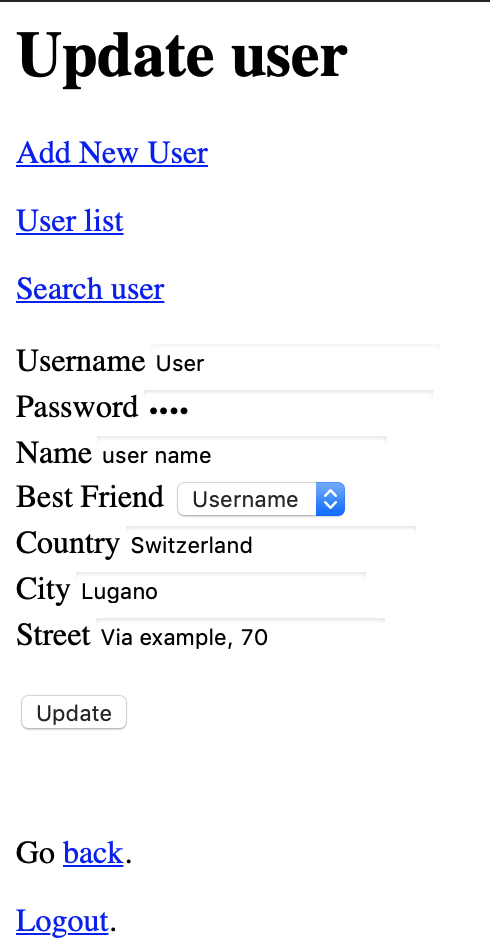
\includegraphics[scale=0.7]{images/updateuser.png}
		\caption{Update user page}
		\label{fig:update_user}
	\end{figure} 
	
	\begin{figure}[ht]
		\centering
		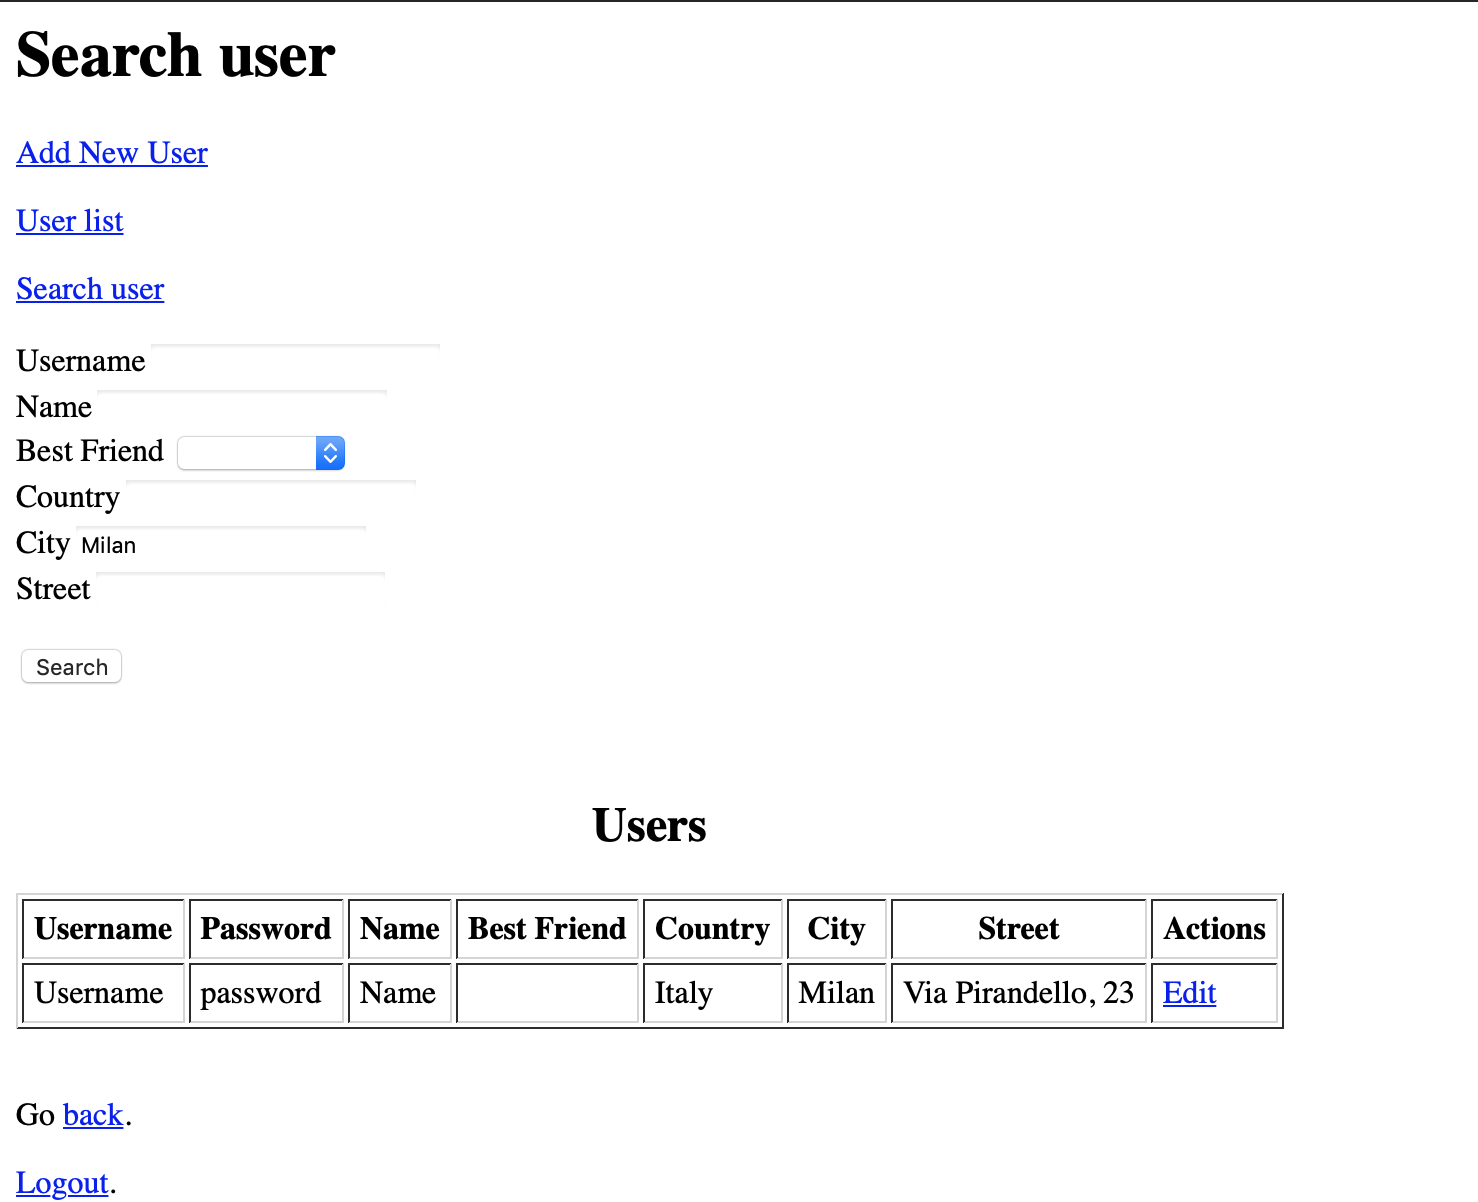
\includegraphics[scale=0.7]{images/usersearch.png}
		\caption{Search user page}
		\label{fig:search_user}
	\end{figure} 
	
	\chapter{Design Patterns}
	\label{cap:design_patterns}
	
	In this chapter a short explaination of (some) used design patterns is given.
	
	\section{Front Controller}
	\label{sec:front_controller}
	
	A single \textit{Front Controller} that handles all requests has been implemented. At the moment it only identifies and delegates the execution to the right command. However, it will be useful in the future to perform common operations like logging, internationalization, etc without duplicating code. It also simplifies the configuration of the server.
	
	\section{Intercepting Filter}
	\label{sec:intercepting_filter}

	An \textit{Intercepting Filter} has been used to manipulate all the requests, preventively checking if the user is authenticated and allowed to visit the requested page. He is redirected to the login page otherwise.
	
	\section{Template view}
	\label{sec:template_view}
	
	HTML code is generated via templates that call proper helpers to get and render data. This easy approach allows the separation of view and implementation logic.
	
	\section{Data Mapper}
	\label{sec:data_mapper}
	
	\texttt{Hibernate} uses the \textit{Data Mapper} pattern to deal with the database, convert objects into rows and vice versa. In fact, it is the one that knows the configuration of the database and relies on a DB layer.
	
	\section{Repository pattern}
	\label{sec:repository_pattern}
	
	The \textit{Respository pattern} has been used to create a layer that deals with the \textit{Data Mapper}, encapsulating logic required to access data sources and separating it from the business one. In this way common data access functionalities are centralized and it is possible to change persistence technology in an easier way. It improves also the maintainability and decoupling of the whole software infrastructure.
	
	\section{Identity Field}
	\label{sec:identity_field}
	
	In order to pair in-memory and DB object identities the \textit{Identity Field} pattern has been used. In the database, the \texttt{users} table has a primary key constraint on the \texttt{username} column while in the model there is a \texttt{String} attribute that maps the \texttt{username} itself. In the case of the \texttt{Address} entity, an identity integer field representing the \texttt{id} is present.
	
	\section{Lazy Load}
	\label{sec:lazy_load}
	
	As specified in the requirements, each user might have a best friend. This is represented with an attribute in the model and translated with a relationship at the database level. When we fetch a user, it is not convenient to fetch also his best friend, since this procedure can be transitive and might end up with the fetching of the entire database (if everyone has a best friend and everyone is referenced).\\
	For this reason, best friends can be fetched only if needed using the \textit{Lazy Load} pattern. Fetching a single user will never cause a lot of useless allocations and data transfers.
	
	\section{Unit of work with Transactional Behaviour}
	\label{sec:unit_of_work_transactional}
	
	\textit{Unit of Work} can be seen into the \texttt{UserRepository} class, all changes are actuated in a transactional way using \texttt{Hibernate} APIs, even though in the given application there are no complex mechanisms to store, delete and update data.
	
	%%%%%%%%%%%%%%%%%%%%%%%%%%%%%%%%%%%%%%%%%%%%%%%%%%%%%  
	\chapter{Architecture}
	\label{cap:architecture}
	
	A high-level architecture of the system is presented in this chapter. A general diagram is provided in figure \ref{fig:general_diagram} and a detailed explanation of its major subparts is provided in every subchapter. It is important to underline that diagrams are also available on the GitHub repository, to download and see them in a more comfortable way. How it has been specified in chapter \ref{sec:resources}.
	
	\section{Authentication}
	\label{sec:authentication}
	
	Authentication is managed by an \textit{Intercepting Filter} named \texttt{AuthFilter}. It is responsible to identify the command that will handle the request (through the \texttt{FrontController}) and check the presence of an \texttt{@Authorize} annotation. Commands without the annotation can serve pages to everyone while commands with the annotation can be accessed only by logged users. This means that the filter is responsible to ensure it via the \texttt{AuthManager} and redirect to the login page otherwise.\\
	It has been decided to use an annotation on every command to promote a declarative way of programming instead of an imperative one.
	
	\section{Repository pattern}
	\label{sec:repository}
	
	A single repository is responsible to perform CRUD operations on the database using \texttt{Hibernate} APIs, as we can see in figure \ref{fig:repository_diagram}. It can be noticed that certain commands call directly the repository while others instantiate helpers that will be later provided to the views. Firsts are usually endpoints of HTML forms that must perform create/update/delete actions while seconds are usually commands that must show information. It is certainly possible to create helpers also to perform the first kind of operation but that logic should be kept well isolated from the view.
	
	\section{Views and Helpers}
	\label{sec:views_and_helpers}
	
	As explained in chapter \ref{sec:template_view} the application uses the \textit{Template View} pattern to generate HTML code. JSP files call methods defined in helper classes to get and render data. These helpers are able to call the repository to interact and perform operations on the database. Obviously, models are then used by every class. The corresponding diagram is shown in figure \ref{fig:helpers_diagram}.
	
	\begin{sidewaysfigure}[ht]
		\centering
		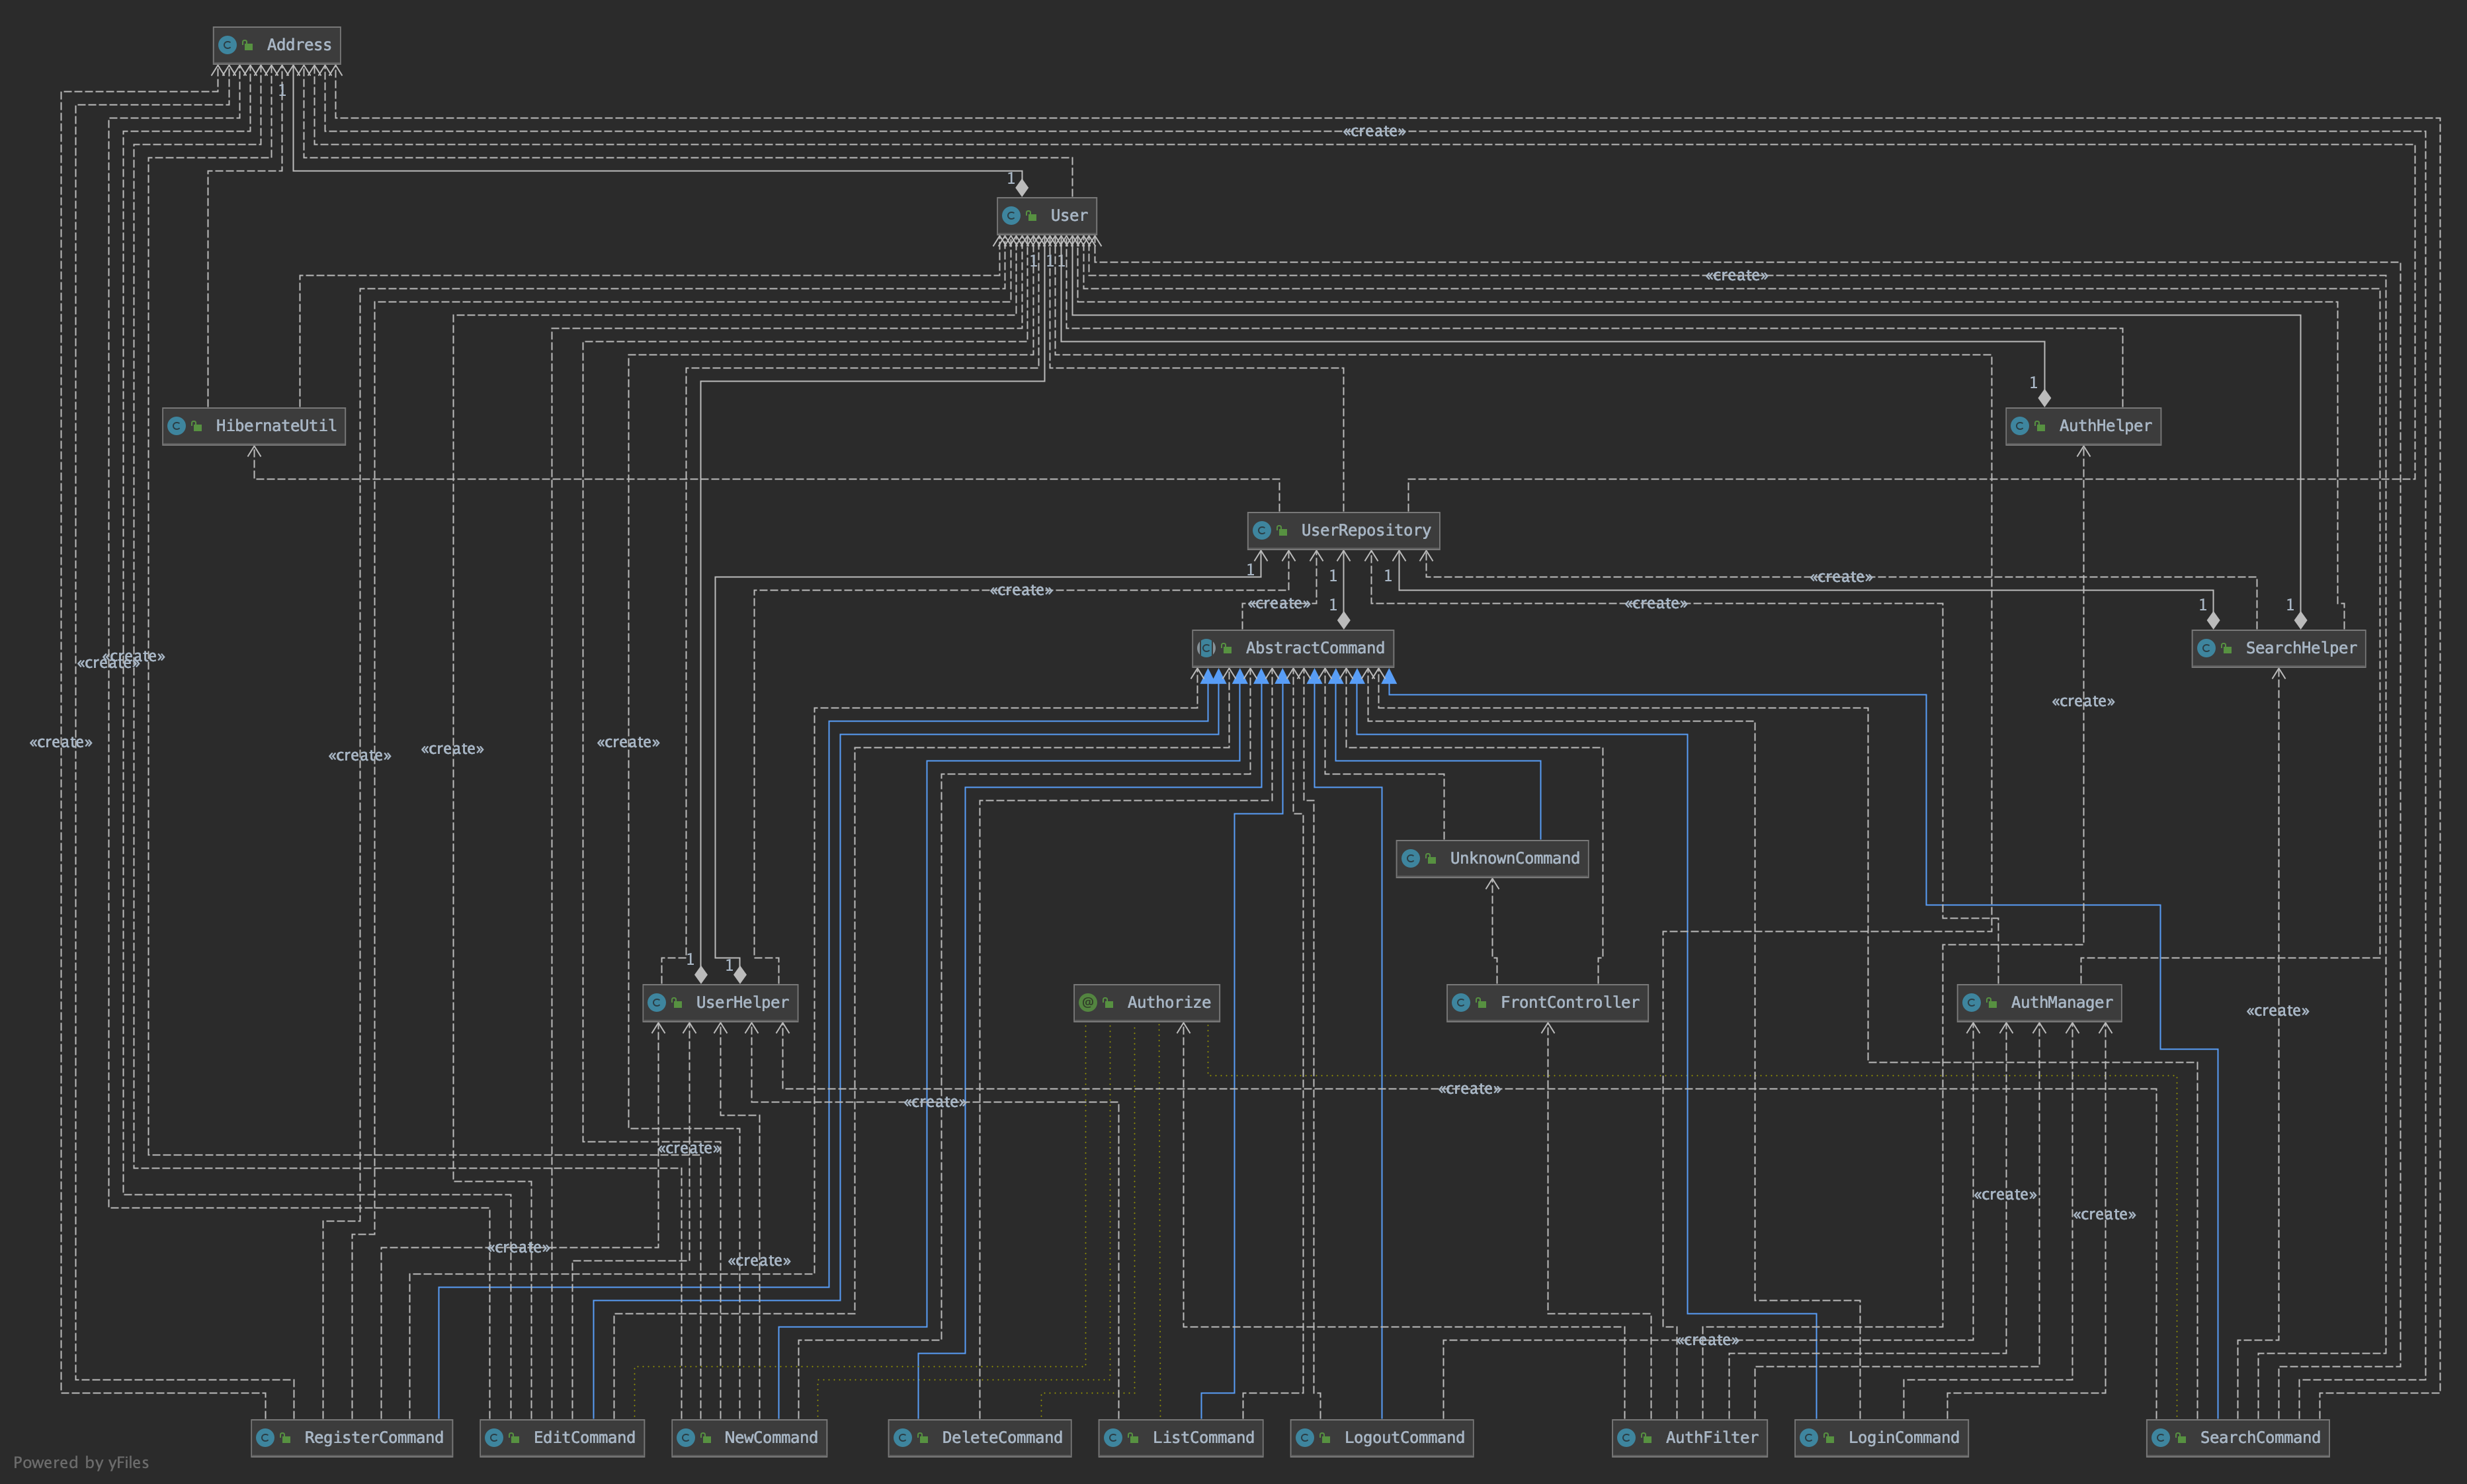
\includegraphics[width=\textwidth]{images/General.png}
		\caption{General diagram}
		\label{fig:general_diagram}
	\end{sidewaysfigure} 
	
	\begin{sidewaysfigure}[ht]
		\centering
		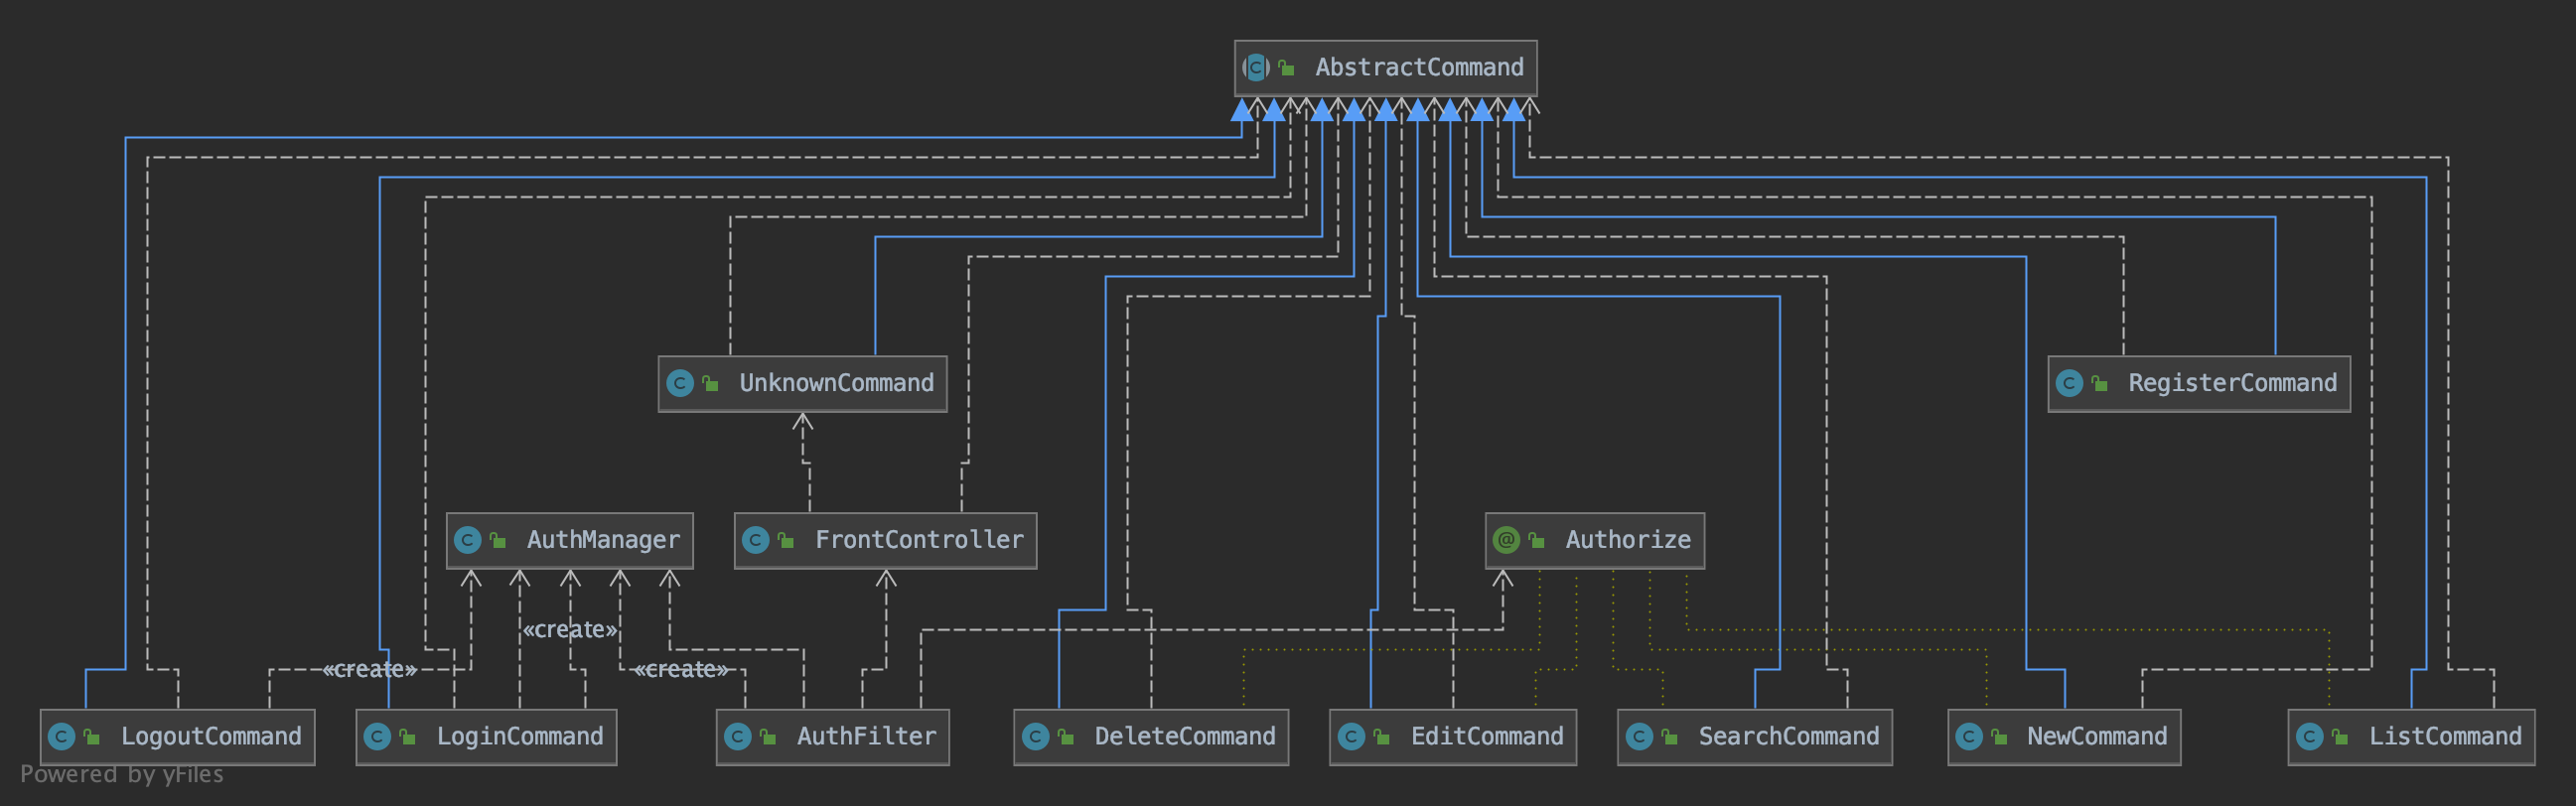
\includegraphics[width=\textwidth]{images/Auth.png}
		\caption{Authentication diagram}
		\label{fig:auth_diagram}
	\end{sidewaysfigure} 
	
	\begin{sidewaysfigure}[ht]
		\centering
		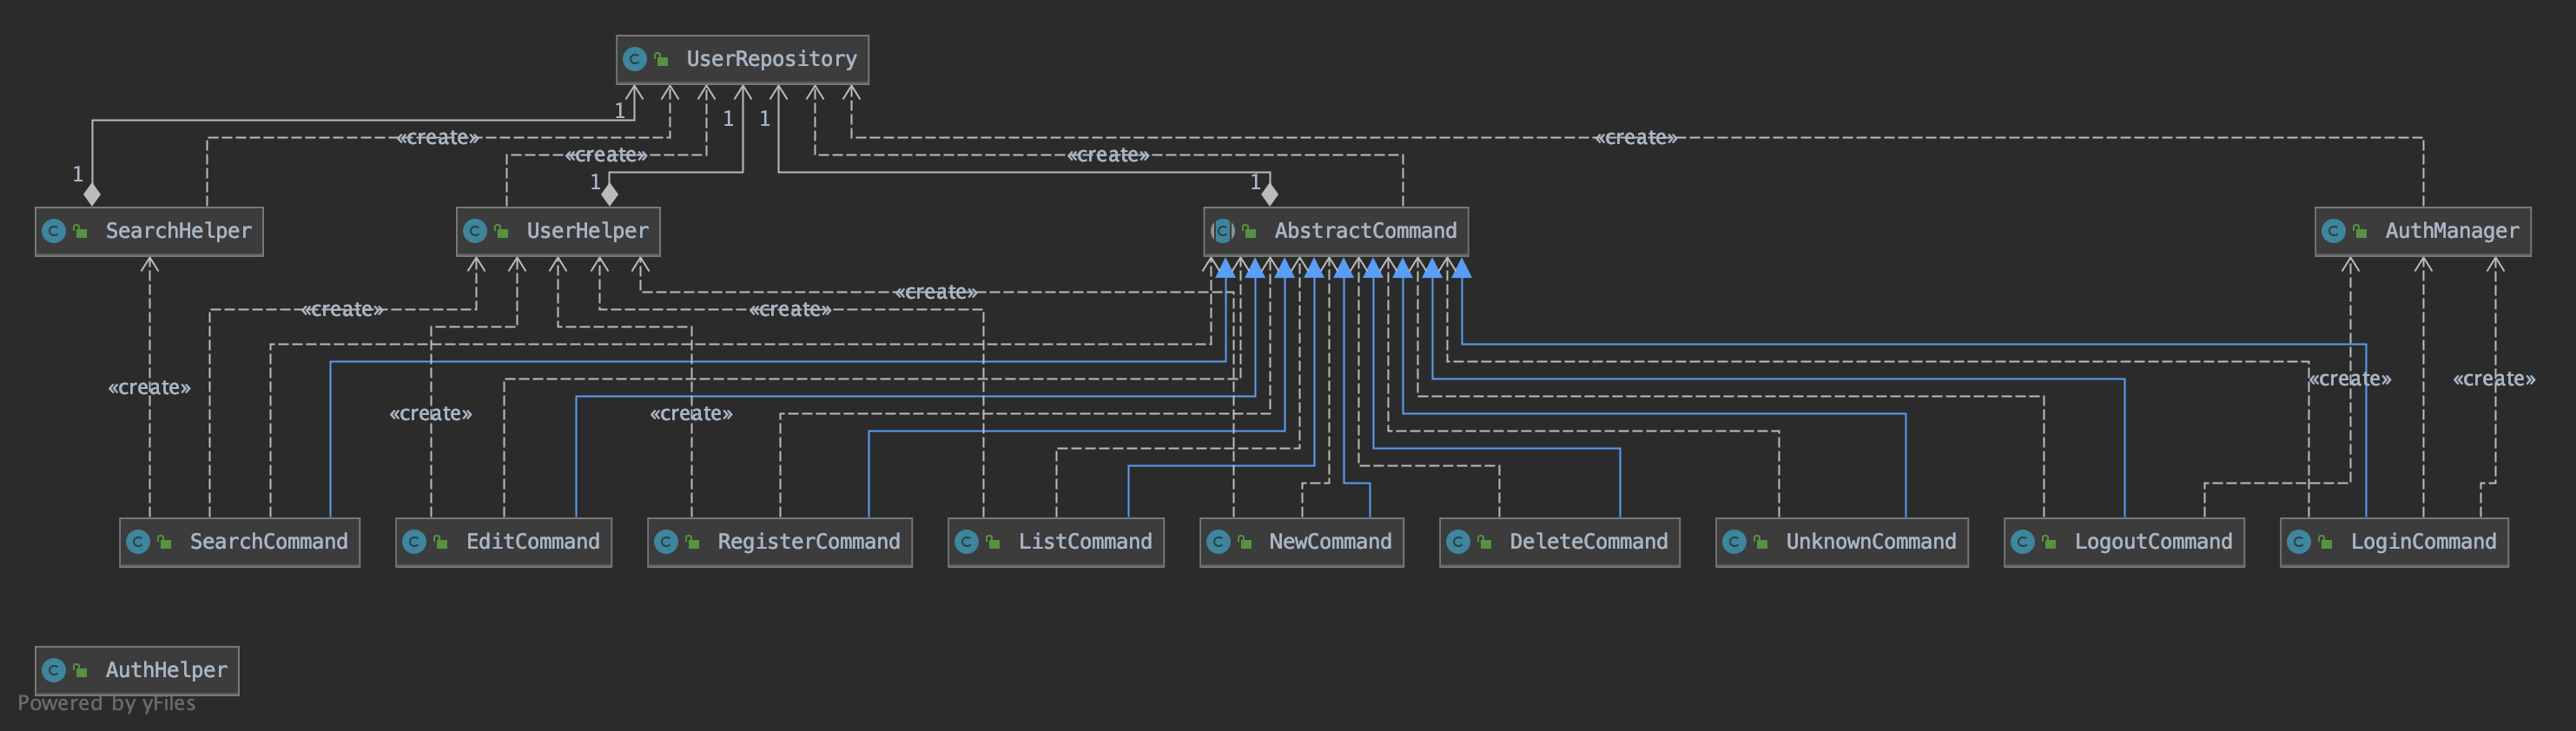
\includegraphics[width=\textwidth]{images/Repository.png}
		\caption{Repository diagram}
		\label{fig:repository_diagram}
	\end{sidewaysfigure} 

	\begin{sidewaysfigure}[ht]
		\centering
		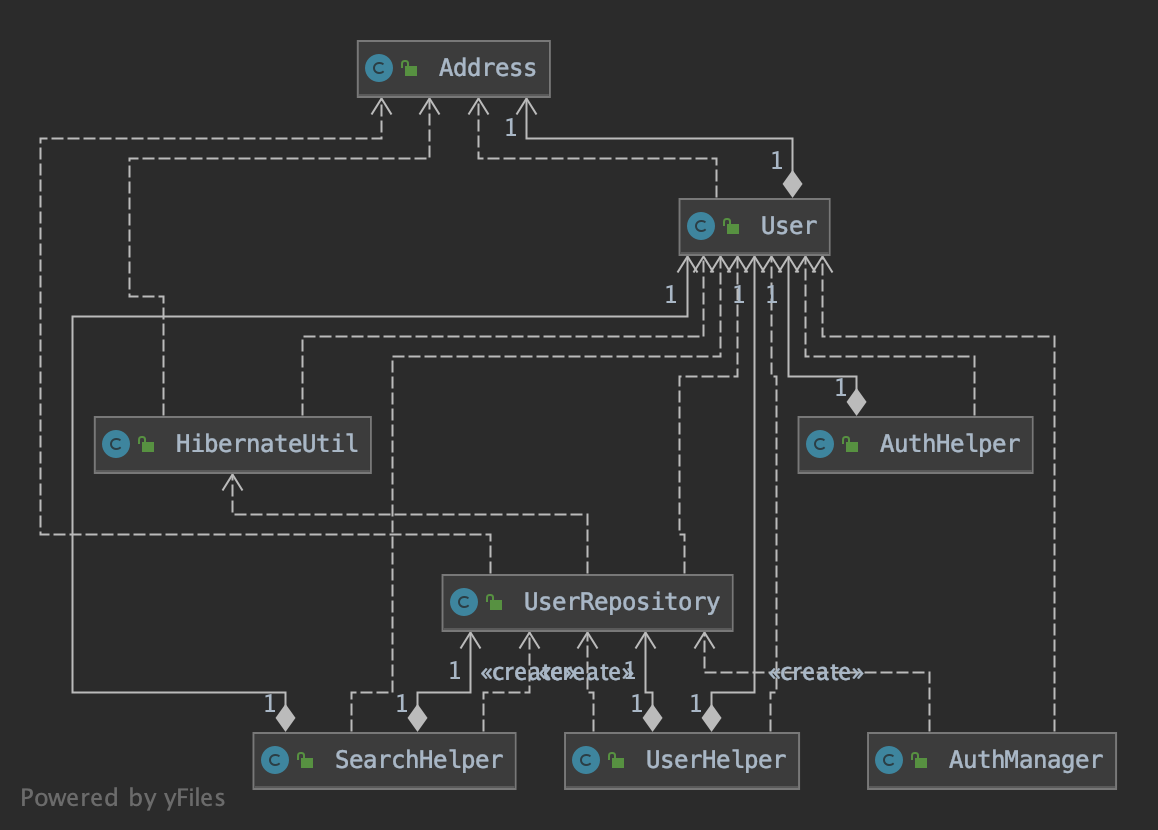
\includegraphics[width=\textwidth]{images/Helpers.png}
		\caption{Helpers diagram}
		\label{fig:helpers_diagram}
	\end{sidewaysfigure} 

	\addcontentsline{toc}{chapter}{Bibliography}
	\printbibliography
	
\end{document}